\documentclass{beamer}

\mode<presentation>
{
    \usetheme{CambridgeUS}
    \usecolortheme{seahorse}
}

\usepackage[french]{babel}
\usepackage[utf8]{inputenc}
\usepackage{sourcesanspro}
\usepackage[T1]{fontenc}
\usepackage{graphicx}
\usepackage{algorithm2e}
\usepackage{mathtools}

\usepackage{url}
\usepackage{hyperref}

\DeclareMathOperator{\diag}{diag}

\definecolor{mauve1}{RGB}{51, 51, 184}
\definecolor{mauve2}{RGB}{214, 214, 240}
\definecolor{mauve3}{RGB}{235, 235, 247}


\newtheorem{thm}{Théorème}
\newtheorem{lem}{Lemme}
\newtheorem{prop}{Proposition}
\newtheorem{defn}{Definition}
\newtheorem{exmp}{Exemple}
\newtheorem{algo}{Algorithme}

\newcommand{\D}{\mathbb{D}}

\setbeamercolor{block title}{fg=mauve1,bg=mauve2}
\setbeamercolor{block body}{bg=mauve3}

\logo{\raisebox{-0.5\height}{
\includegraphics[width=10mm]{unamur.png}}}

\setbeamertemplate{navigation symbols}{}

\setbeamersize{text margin left=7mm}
\setbeamersize{text margin right=7mm}

%\usepackage{ragged2e}
%\apptocmd{\frame}{}{\justifying}{}

\title[Recherche directe et calibration]{{\small \textsc{Présentation des mémoires}} \\ {\scriptsize(Promoteur : \textsc{Franco} Nicolas)}}
\subtitle{\Large Les méthodes de recherche directe pour la calibration d’un modèle épidémiologique} 
\author[\textsc{Foncoux} E.]{\textsc{Foncoux} Esteban}
\institute[UNamur]{}
\date{Octobre 2023}

\begin{document}

\begin{frame}
  \titlepage
\end{frame}

\logo{}

\begin{frame}
    \frametitle{Plan de la présentation}
    \tableofcontents
\end{frame}

\AtBeginSection[]
{
  \begin{frame}
    \frametitle{Plan de la présentation}
    \tableofcontents[currentsection,hideallsubsections]
  \end{frame}
}


\section{Introduction}

\begin{frame}{Introduction}
    \begin{itemize}
        \item Objectif : comprendre et utiliser des méthodes de recherche directe pour calibrer un modèle épidémilogique.
        \item Comparer les résultats avec la méthode de recherche aléatoire.
    \end{itemize}
\end{frame}

\section{Bases positives}

\begin{frame}{Définition}
    \begin{defn}[Combinaison linéaire positive]
        Un vecteur $d$ est une combinaison linéaire positive des vecteurs $\{d_1,d_2,\dots,d_m\}$ si et seulement si 
    $$
        d=\sum_{i=1}^m \alpha_i d_i
    $$
    avec $\alpha_i \geq 0$.
    \end{defn}
    
\end{frame}

\begin{frame}{Définition}
    \begin{defn}[Span positif et générateur positif]
        Soit $\mathbb{D} \subseteq \mathbb{R}^n$. Le span positif de $\mathbb{D}$ est l'ensemble des combinaisons linéaires positives de vecteurs de $\mathbb{D}$ : 
        $$
            pspan(\mathbb{D}) = \left\{ \sum_{i=1}^m \alpha_i d_i | \alpha_i \geq 0, d_i\in\mathbb{D},m\leq n \in \mathbb{N}  \right\} \subseteq \mathbb{R}^n.
        $$
    On dira que $\mathbb{D}$ est générateur positif de $\mathbb{R}^n$ si et seulement si $pspan(\mathbb{D}) = \mathbb{R}^n$.
    \end{defn}
    
\end{frame}

\begin{frame}{Définition}
    \begin{defn}[Indépendance linéaire positive]
        Les vecteurs d'un ensemble $\mathbb{D}$ sont positivement linéairement indépendant si et seulement si $d\not\in pspan(\mathbb{D}\backslash\{d\}), \forall d \in \mathbb{D}$.
    \end{defn}

    \begin{defn}[Base positive]
        Un ensemble $\mathbb{D}$ est une base positive de $\mathbb{R}^n$ si et seulement si cet ensemble est un générateur positif de $\mathbb{R}^n$ et ses vecteurs sont positivement linéairement indépendant.
    \end{defn}
    
\end{frame}

\begin{frame}{Illustration}
    \begin{figure}
    \centering
    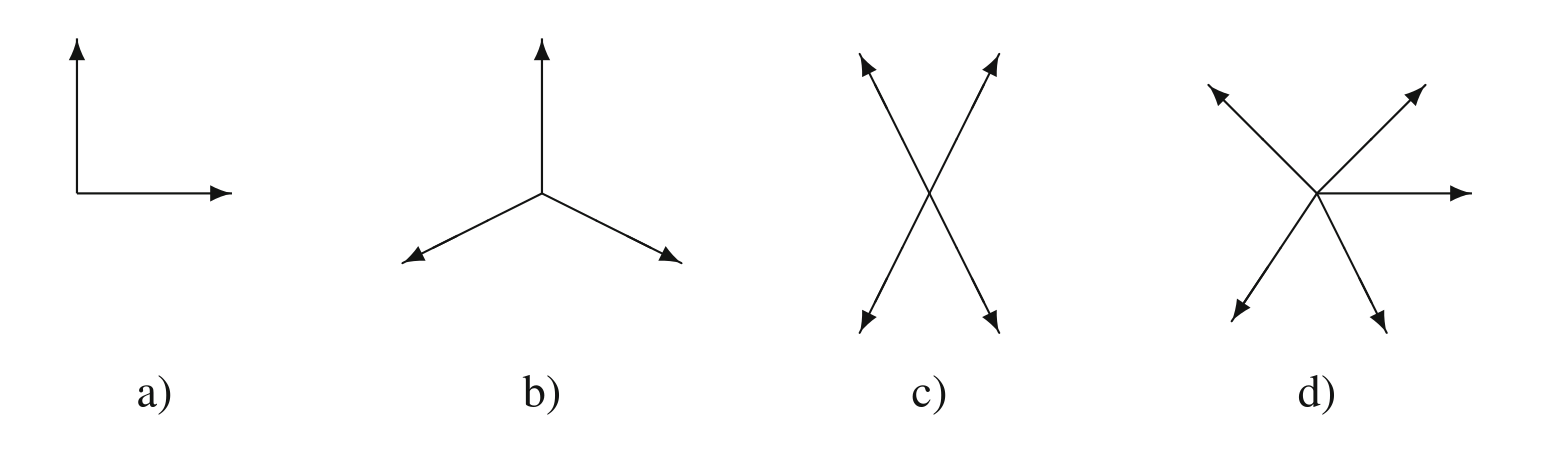
\includegraphics[width = 11cm]{illustration_pspan_pbases.png}
    \caption{Illustration d'une base (a), de 2 bases positives (b), (c) et un span positif (d) dans $\mathbb{R}^2$. Source : \cite{AuHa2017a}.}
    \label{fig:bases,pspan, pLI}
\end{figure}
\end{frame}


\begin{frame}{Base positive et optimisation}
    \begin{thm}[Base positive maximale et minimale]
        Soit $\D$ une base positive de $\mathbb{R}^n$. Alors $\D$ a au moins $n+1$ vecteurs et au plus $2n$ vecteurs.
    \end{thm}
    
    \begin{thm}[Base positive et direction de descente]
        Soit $\D$ un ensemble générateur positif dans $\mathbb{R}^n$ et $w \in \mathbb{R}_0^n$.
    Alors, il existe $d \in \D$ tel que $w^T d < 0$. De plus, si $f \in \mathcal{C}^1$ et $\nabla f(x) \neq 0 $ pour au moins un $x \in \mathbb{R}^n$, alors il existe $d \in \D$ tel que $d$ est une direction de descente de $f$ en $x$.
    \end{thm}

\end{frame}

\section{Optimisation boîte-noire}

\begin{frame}{Concept de boîte-noire}
    \begin{figure}
    \centering
    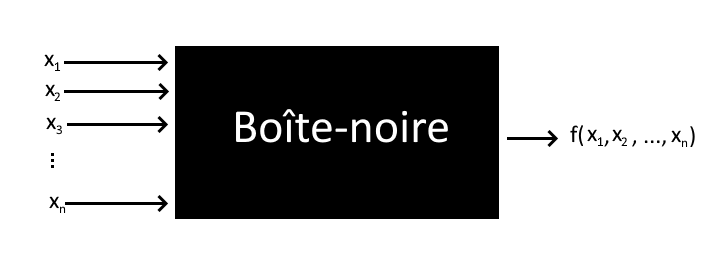
\includegraphics[width=11cm]{blackbox.png}
    \caption{Illustration du concept de boite-noire.}
    \label{fig:blackbox}
\end{figure}
\end{frame}

\begin{frame}{Classification}
    \begin{figure}[htbp]
    \centering
    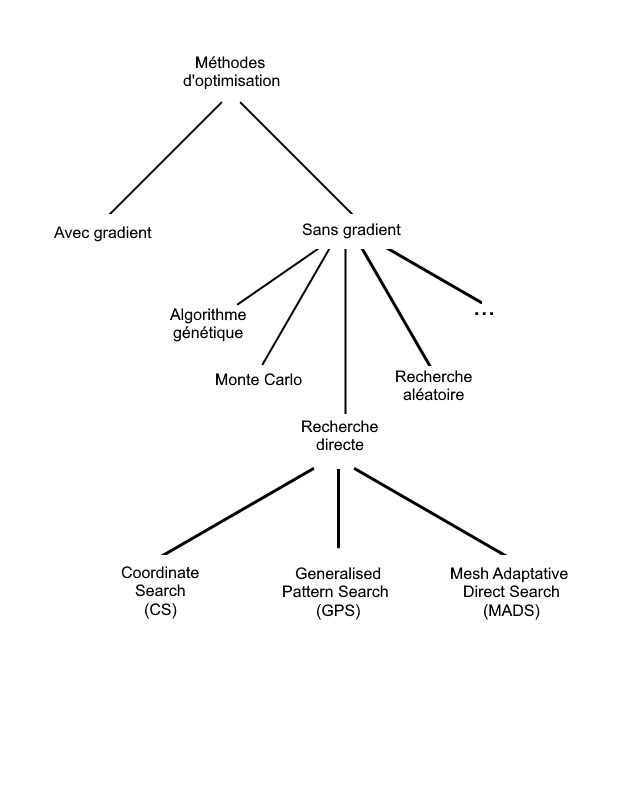
\includegraphics[width=7.5cm]{classification.png}
    \caption{Classification de différentes méthodes d'optimisation selon l'utilisation ou non du gradient.}
    \label{fig:classification_methode_opti}
\end{figure}
\end{frame}



\section{Algorithme de recherche directe}

\begin{frame}{Coordinate Search (CS)}
    \begin{figure}[htbp]
    \centering
    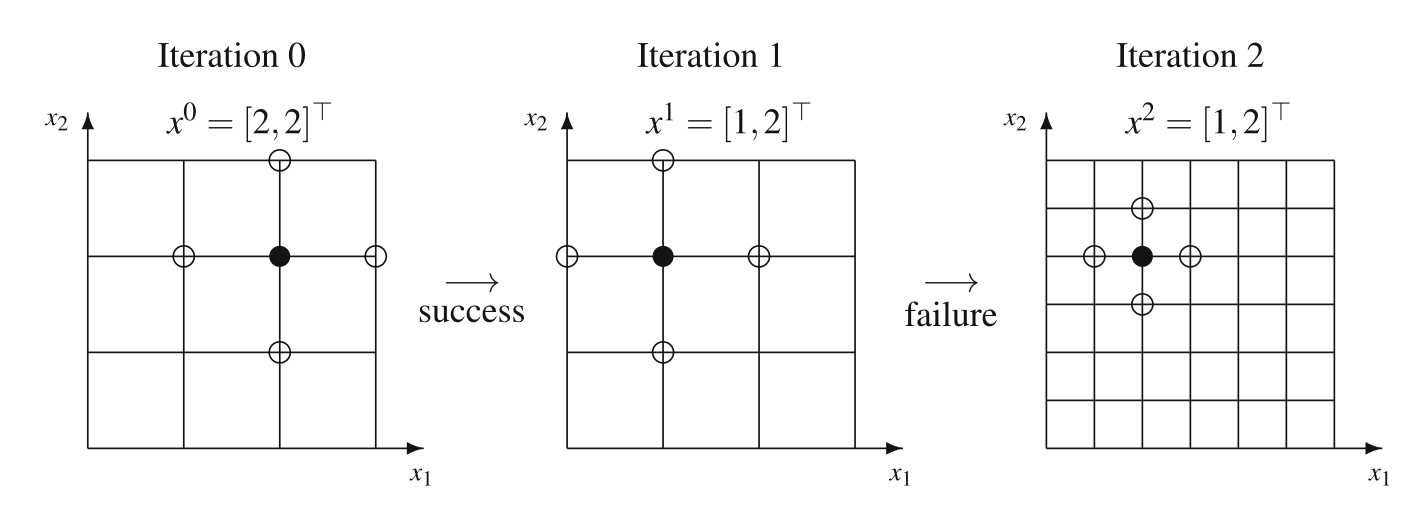
\includegraphics[width=11cm]{CS_algo_illustration.png}
    \caption{Illustration de l'algorithme CS dans $\mathbb{R}^2$. Source : \cite{AuHa2017a}.}
    \label{fig:CS}
\end{figure}
\end{frame}


\begin{frame}{Generalised Pattern Search (GPS)}
    \begin{figure}[htbp]
        \centering
        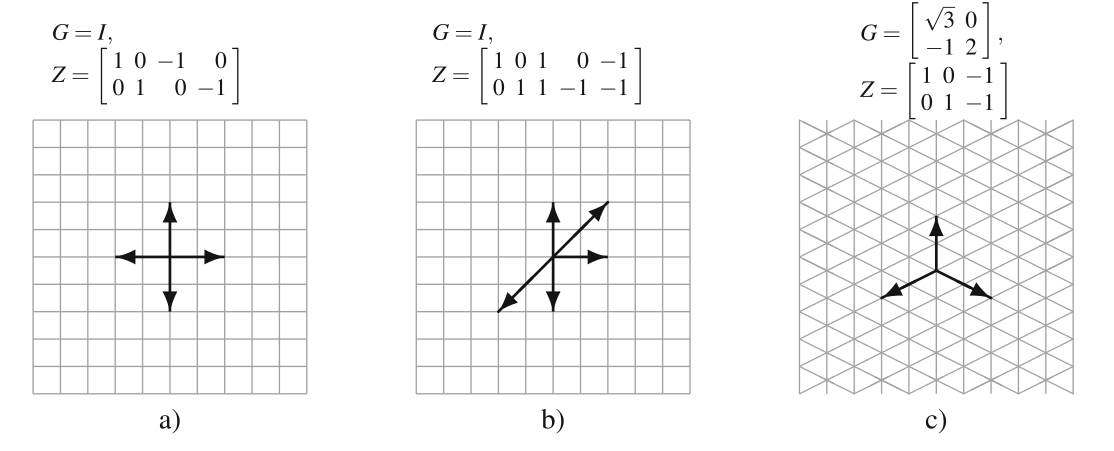
\includegraphics[width=11cm]{GPS_GZ.png}
        \caption{Représentation de l'impact des matrices $G$ et $Z$ dans $\mathbb{R}^2$ avec $\delta^k=\frac{1}{2}$ sur la structure du maillage et l'ensemble des directions. Source : \cite{AuHa2017a}.}
        \label{fig:GPS GZ}
    \end{figure}
\end{frame}

\begin{frame}{Mesh Adaptative Direct Search (MADS)}
    \begin{figure}
    \centering
    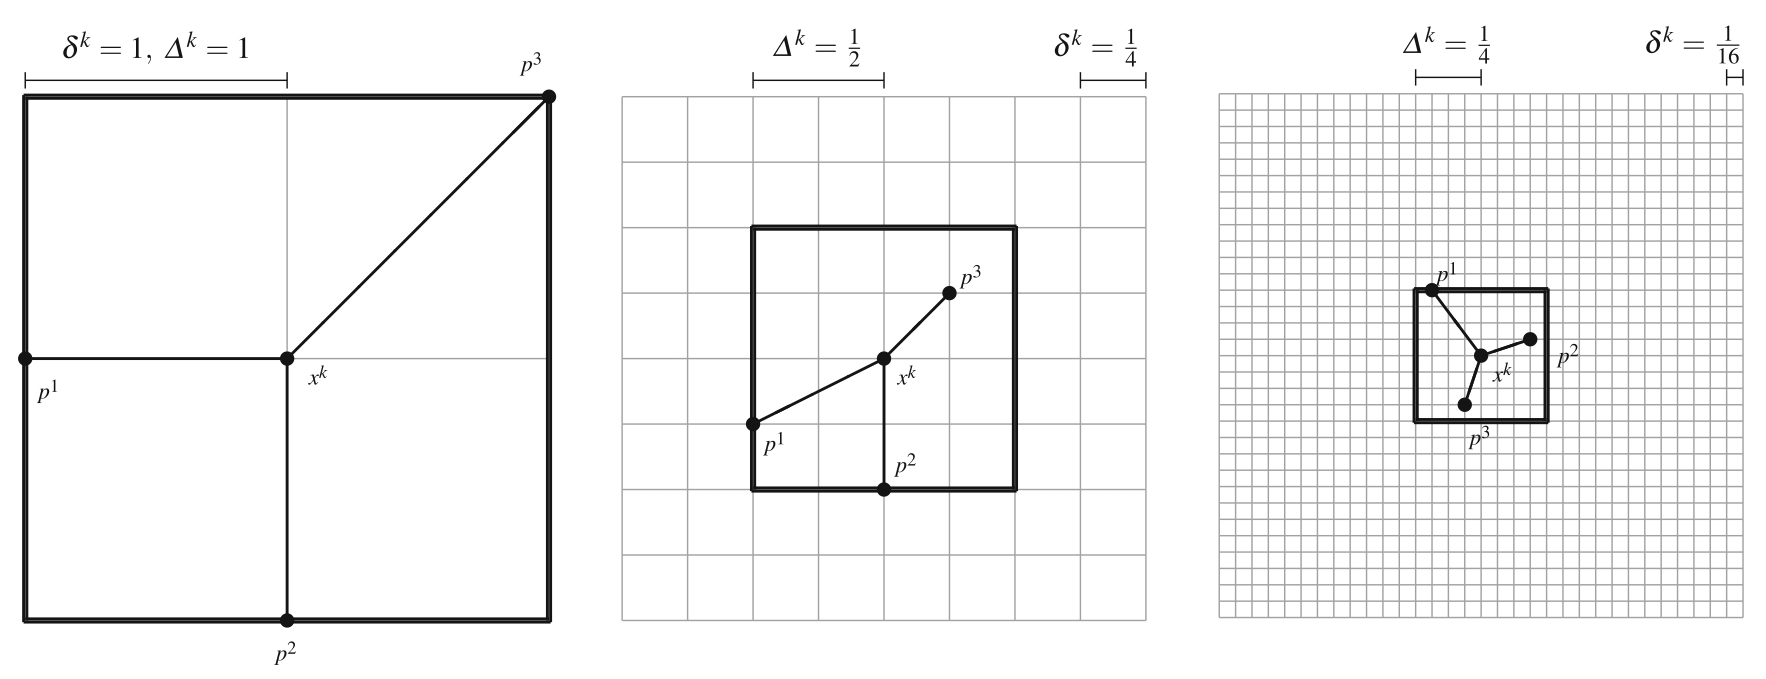
\includegraphics[width=11.2cm]{MADS_illustration_beamer.jpg}
    \caption{Illustration du maillage et du cadre selon différentes valeurs du paramètre de taille de maillage $\delta^k$ et de cadre $\delta^k$. Source : \cite{AuHa2017a}.}
    \label{fig:MADS illustration}
\end{figure}
\end{frame}

\section{Conclusion et perspective}
\begin{frame}{Conclusion et perspective}

    \begin{itemize}
        \item Approfondir le concept de boîte-noire et d'optimisation (avec et sans contraintes).
        \item Expliciter les particularités des algorithmes CS, GPS et MADS.
        \item Construire un modèle épidémiologique et l'expliquer.
        \item Comparer les résultats.
        
    \end{itemize}
    
\end{frame}

\begin{frame}{Bibliographie}
    \bibliographystyle{apalike2}
    \bibliography{sources}
    
\end{frame}

\end{document}
